\documentclass[journal, a4paper]{Spades_Logic_Dependency/IEEEtran}

% some very useful LaTeX packages include:

%\usepackage{cite}      % Written by Donald Arseneau
                        % V1.6 and later of IEEEtran pre-defines the format
                        % of the cite.sty package \cite{} output to follow
                        % that of IEEE. Loading the cite package will
                        % result in citation numbers being automatically
                        % sorted and properly "ranged". i.e.,
                        % [1], [9], [2], [7], [5], [6]
                        % (without using cite.sty)
                        % will become:
                        % [1], [2], [5]--[7], [9] (using cite.sty)
                        % cite.sty's \cite will automatically add leading
                        % space, if needed. Use cite.sty's noadjust option
                        % (cite.sty V3.8 and later) if you want to turn this
                        % off. cite.sty is already installed on most LaTeX
                        % systems. The latest version can be obtained at:
                        % http://www.ctan.org/tex-archive/macros/latex/contrib/supported/cite/

\usepackage{graphicx}   % Written by David Carlisle and Sebastian Rahtz
                        % Required if you want graphics, photos, etc.
                        % graphicx.sty is already installed on most LaTeX
                        % systems. The latest version and documentation can
                        % be obtained at:
                        % http://www.ctan.org/tex-archive/macros/latex/required/graphics/
                        % Another good source of documentation is "Using
                        % Imported Graphics in LaTeX2e" by Keith Reckdahl
                        % which can be found as esplatex.ps and epslatex.pdf
                        % at: http://www.ctan.org/tex-archive/info/

%\usepackage{psfrag}    % Written by Craig Barratt, Michael C. Grant,
                        % and David Carlisle
                        % This package allows you to substitute LaTeX
                        % commands for text in imported EPS graphic files.
                        % In this way, LaTeX symbols can be placed into
                        % graphics that have been generated by other
                        % applications. You must use latex->dvips->ps2pdf
                        % workflow (not direct pdf output from pdflatex) if
                        % you wish to use this capability because it works
                        % via some PostScript tricks. Alternatively, the
                        % graphics could be processed as separate files via
                        % psfrag and dvips, then converted to PDF for
                        % inclusion in the main file which uses pdflatex.
                        % Docs are in "The PSfrag System" by Michael C. Grant
                        % and David Carlisle. There is also some information
                        % about using psfrag in "Using Imported Graphics in
                        % LaTeX2e" by Keith Reckdahl which documents the
                        % graphicx package (see above). The psfrag package
                        % and documentation can be obtained at:
                        % http://www.ctan.org/tex-archive/macros/latex/contrib/supported/psfrag/

%\usepackage{subfigure} % Written by Steven Douglas Cochran
                        % This package makes it easy to put subfigures
                        % in your figures. i.e., "figure 1a and 1b"
                        % Docs are in "Using Imported Graphics in LaTeX2e"
                        % by Keith Reckdahl which also documents the graphicx
                        % package (see above). subfigure.sty is already
                        % installed on most LaTeX systems. The latest version
                        % and documentation can be obtained at:
                        % http://www.ctan.org/tex-archive/macros/latex/contrib/supported/subfigure/

\usepackage{url}        % Written by Donald Arseneau
                        % Provides better support for handling and breaking
                        % URLs. url.sty is already installed on most LaTeX
                        % systems. The latest version can be obtained at:
                        % http://www.ctan.org/tex-archive/macros/latex/contrib/other/misc/
                        % Read the url.sty source comments for usage information.

%\usepackage{stfloats}  % Written by Sigitas Tolusis
                        % Gives LaTeX2e the ability to do double column
                        % floats at the bottom of the page as well as the top.
                        % (e.g., "\begin{figure*}[!b]" is not normally
                        % possible in LaTeX2e). This is an invasive package
                        % which rewrites many portions of the LaTeX2e output
                        % routines. It may not work with other packages that
                        % modify the LaTeX2e output routine and/or with other
                        % versions of LaTeX. The latest version and
                        % documentation can be obtained at:
                        % http://www.ctan.org/tex-archive/macros/latex/contrib/supported/sttools/
                        % Documentation is contained in the stfloats.sty
                        % comments as well as in the presfull.pdf file.
                        % Do not use the stfloats baselinefloat ability as
                        % IEEE does not allow \baselineskip to stretch.
                        % Authors submitting work to the IEEE should note
                        % that IEEE rarely uses double column equations and
                        % that authors should try to avoid such use.
                        % Do not be tempted to use the cuted.sty or
                        % midfloat.sty package (by the same author) as IEEE
                        % does not format its papers in such ways.

\usepackage{amsmath}    % From the American Mathematical Society
                        % A popular package that provides many helpful commands
                        % for dealing with mathematics. Note that the AMSmath
                        % package sets \interdisplaylinepenalty to 10000 thus
                        % preventing page breaks from occurring within multiline
                        % equations. Use:
%\interdisplaylinepenalty=2500
                        % after loading amsmath to restore such page breaks
                        % as IEEEtran.cls normally does. amsmath.sty is already
                        % installed on most LaTeX systems. The latest version
                        % and documentation can be obtained at:
                        % http://www.ctan.org/tex-archive/macros/latex/required/amslatex/math/



% Other popular packages for formatting tables and equations include:

%\usepackage{array}
% Frank Mittelbach's and David Carlisle's array.sty which improves the
% LaTeX2e array and tabular environments to provide better appearances and
% additional user controls. array.sty is already installed on most systems.
% The latest version and documentation can be obtained at:
% http://www.ctan.org/tex-archive/macros/latex/required/tools/

% V1.6 of IEEEtran contains the IEEEeqnarray family of commands that can
% be used to generate multiline equations as well as matrices, tables, etc.

% Also of notable interest:
% Scott Pakin's eqparbox package for creating (automatically sized) equal
% width boxes. Available:
% http://www.ctan.org/tex-archive/macros/latex/contrib/supported/eqparbox/

% *** Do not adjust lengths that control margins, column widths, etc. ***
% *** Do not use packages that alter fonts (such as pslatex).         ***
% There should be no need to do such things with IEEEtran.cls V1.6 and later.


% Your document starts here!
\begin{document}

% Define document title and author
	\title{Spades Logic}
	\author{Project Vegas
	\thanks{Adam, Dave, Matt, Scott}}
	\markboth{CS 3450}{}
	\maketitle

% Write abstract here


% Each section begins with a \section{title} command
\section{Introduction}
	% \PARstart{}{} creates a tall first letter for this first paragraph
	\PARstart{S}{pades} is a trick-taking card game devised in the United States in the 1930s. It can be played as either a partnership or solo/"cutthroat" game. The object is to take at least the number of tricks (also known as "books") that were bid before play of the hand began. Spades is a descendant of the Whist family of card games, which also includes Bridge, Hearts, and Oh Hell. Its major difference as compared to other Whist variants is that, instead of trump being decided by the highest bidder or at random, the Spade suit is always trumps, hence the name. (Wikipedia)

% Main Part
\section{Rules}
	
\textbf{The Pack} \newline
The standard 52-card pack is used.\newline

\textbf{Rank of Suits} \newline
The spade suit is always trump.\newline

\textbf{Rank of Cards}\newline
A (high), K, Q, J, 10, 9, 8, 7, 6, 5, 4, 3, 2.\newline

\textbf{Object of the Game}\newline
To win at least the number of tricks bid.\newline

\textbf{The Deal} \newline
The first dealer is chosen by a draw for high card, and thereafter the turn to deal proceeds clockwise. The entire deck is dealt one at a time, face down, beginning on the dealer's left. The players then pick up their cards and arrange them by suits.
The Bidding

Each player decides how many tricks he will be able to take. The player to the dealer's left starts the bidding and, in turn, each player states how many tricks he expects to win. There is only one round of bidding, and the minimum bid is One. Every player must make a bid; no player may pass. No suit is named in the bid, for as the name of the game implies, spades are always trump.\newline

\textbf{The Play}\newline
The game is scored by hands, and the winner must make a certain number of points, which is decided before the game begins. Five hundred points is common, but 200 points is suitable for a short game. The player on the dealer's left makes the opening lead, and players must follow suit, if possible. If a player cannot follow suit, he may play a trump or discard. The trick is won by the player who plays the highest trump or if no trump was played, the player who played the highest card in the suit led. The player who wins the trick leads next. Play continues until none of the players have any cards left. Each hand is worth 13 tricks. Spades cannot be led unless played previously or player to lead has nothing but Spades in his hand.
How to Keep Score

For making the contract (the number of tricks bid), the player scores 10 points for each trick bid, plus 1 point for each overtrick.

For example, if the player's bid is Seven and he makes seven tricks, the score would be 70. If the bid was Five and the player won eight tricks, the score would be 53 points: 50 points for the bid, and 3 points for the three overtricks. In some games, overtricks are called "bags" and a deduction of 100 points is made every time a player accumulates 10 bags. Thus, the object is always to fulfill the bid exactly.

If the player "breaks contract," that is, if he takes fewer than the number of tricks bid, the score is 0. For example, if a player bids Four and wins only three tricks, no points are awarded.
One of the players is the scorer and writes the bids down, so that during the play and for the scoring afterward, this information will be available to all the players. When a hand is over, the scores should be recorded next to the bids, and a running score should be kept so that players can readily see each other's total points. If there is a tie, then all players participate in one more round of play. (bicyclecards.com)


\section{Logic}
	
	% This is how you define a table: the [!hbt] means that LaTeX is forced (by the !) to place the table exactly here (by h), or if that doesnt work because of a pagebreak or so, it tries to place the table to the bottom of the page (by b) or the top (by t).

	% If you have questions about how to write mathematical formulas in LaTeX, please read a LaTeX book or the 'Not So Short Introduction to LaTeX': tobi.oetiker.ch/lshort/lshort.pdf

	% This is how you include a eps figure in your document. LaTeX only accepts EPS or TIFF files.

	
	\begin{figure}[!hbt]
		% Center the figure.
		\begin{center}
		% Include the eps file, scale it such that it's width equals the column width. You can also put width=8cm for example...
		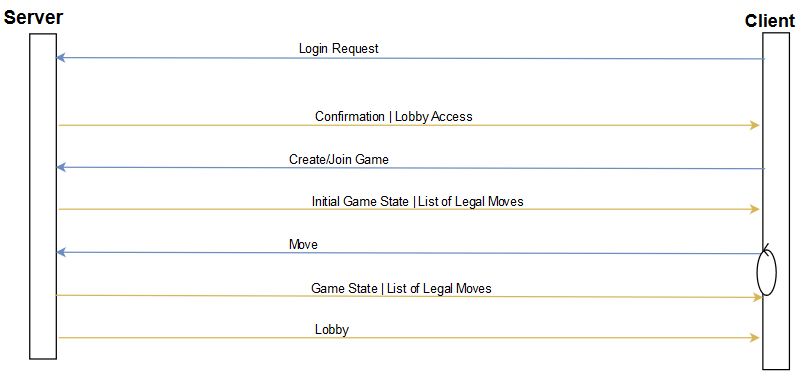
\includegraphics[width=\columnwidth]{graphics/clientServer}
		% Create a subtitle for the figure.
		\caption{Server - Client model for spades.}
		% Define the label of the figure. It's good to use 'fig:title', so you know that the label belongs to a figure.
		\label{Figure 1}
		\end{center}
	\end{figure}
	
	As we are dealing with a \textbf{thin client | fat server} model, figure 1 outlines the general idea behind communication required for the game of Spades. The client will initialize the process with a login request. After which \textit{(assuming success)} the server will reply and grant the client access to the game lobby. The client will either attempt to join a game or instantiate a new one. After the game is fully set up the game initializes a loop handing the client - server for the remainder of the game. The server sends the state of the game along with a list of legal moves. The client will reply. This process will continue until the game is either interrupted or completed. After which, the server grants access to the lobby.  
	
		\begin{figure}[!hbt]
		% Center the figure.
		\begin{center}
		% Include the eps file, scale it such that it's width equals the column width. You can also put width=8cm for example...
		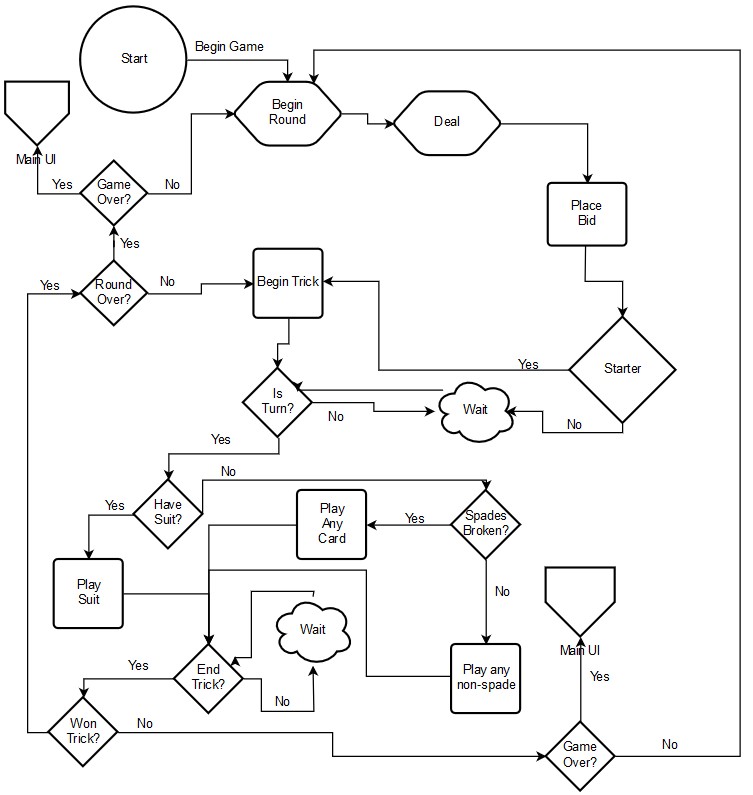
\includegraphics[width=\columnwidth]{graphics/logicDiagram}
		% Create a subtitle for the figure.
		\caption{Activity diagram for spades.}
		% Define the label of the figure. It's good to use 'fig:title', so you know that the label belongs to a figure.
		\label{Figure 1}
		\end{center}
	\end{figure}
	

\section{Conclusion}
	Spades is a fun game. 

% Now we need a bibliography:
\begin{thebibliography}{5}

	%Each item starts with a \bibitem{reference} command and the details thereafter.
	\bibitem{HOP96} % Transaction paper
	http://www.bicyclecards.com/how-to-play/spades/ 

	\bibitem{MJH06} % Conference paper
	https://en.wikipedia.org/wiki/Spades

\end{thebibliography}

% Your document ends here!
\end{document}